\begin{figure*}[!h]
\begin{subfigure}{0.20\linewidth}
\centering
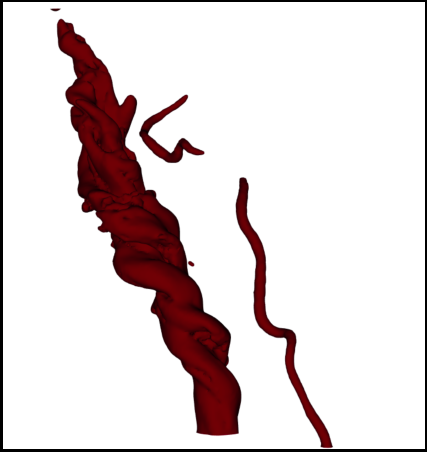
\includegraphics[width=0.9\linewidth]{Images/Tornado/zls.pdf}
\vspace{-2mm}
\caption{$ZLS_{T}$}
\label{fig:tornado_zls}
\end{subfigure}
\begin{subfigure}{0.20\linewidth}
\centering
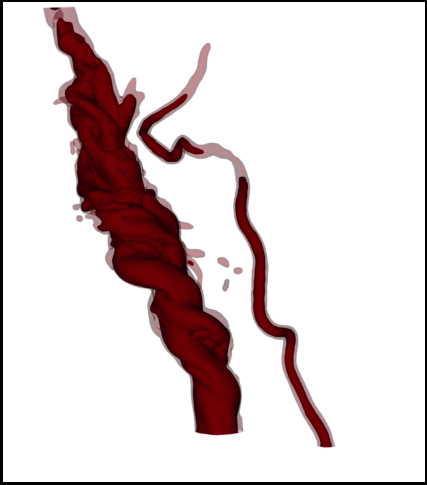
\includegraphics[width=0.9\linewidth]{Images/Tornado/fcls_50.pdf}
\vspace{-2mm}
\caption{+ $FCLS_{T,50\%}$}
\label{fig:tornado_fls}
\end{subfigure}
\begin{subfigure}{0.20\linewidth}
\centering
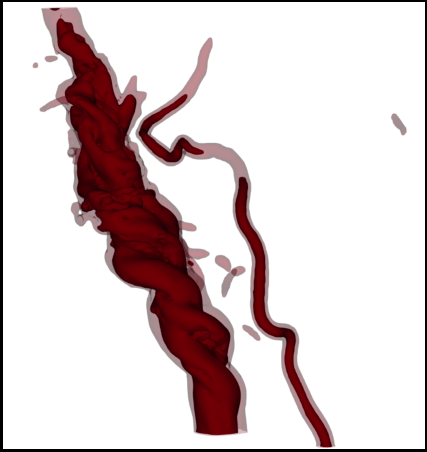
\includegraphics[width=0.9\linewidth]{Images/Tornado/fcls_68.pdf}
\vspace{-2mm}
\caption{+ $FCLS_{T,68\%}$}
\label{fig:tornado_fls}
\end{subfigure}
\begin{subfigure}{0.20\linewidth}
\centering
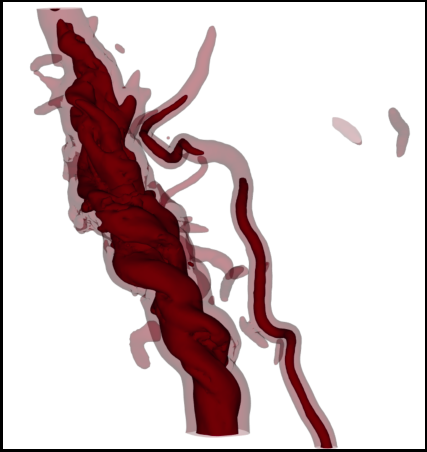
\includegraphics[width=0.9\linewidth]{Images/Tornado/fcls_95.pdf}
\vspace{-2mm}
\caption{+ $FCLS_{T,95\%}$}
\label{fig:tornado_fcls}
\end{subfigure}
\hfill
\begin{subfigure}{0.17\linewidth}
\centering
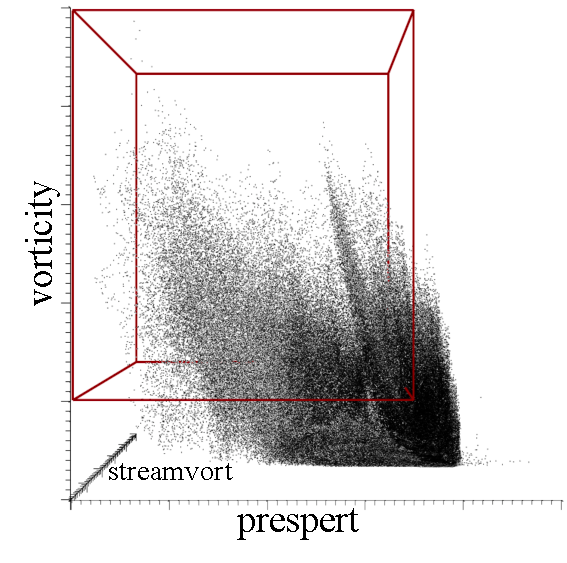
\includegraphics[width=\linewidth]{Images/Tornado/scatterplot3d.pdf}
\vspace{-4mm}
\caption{3D scatterplot of $\mathcal{A}$ and $T$ (red cuboid).} 
\label{fig:tornado_scatterplot}
\end{subfigure}
\vspace{-2mm}
\caption{Visualization of EF-5 tornado vortices using \textit{vorticity}, \textit{prespert} and \textit{streamvort} attributes. As in Figure~\ref{fig:tangle}, $FCLS_{T,C}$ formed wider envelopes as $C$ increased. Importantly, $FCLS_{T,C}$ visualized vortical structures of interest in the vicinity of the primary tornado vortex.}
%\vspace{-1mm}
\label{fig:tornado}
\end{figure*}
